\documentclass[11pt,a4paper]{article}
\usepackage[margin=18mm,top=22mm,bottom=20mm]{geometry}
\usepackage{fontspec}\setmainfont{Latin Modern Roman}
\usepackage{amsmath,amssymb,tikz,graphicx,fancyhdr,array,needspace}
\usetikzlibrary{patterns,arrows.meta,decorations.pathmorphing,calc}
\setlength{\headheight}{14pt}
\usetikzlibrary{arrows.meta}
\pagestyle{fancy}\fancyhf{}\renewcommand{\headrulewidth}{0.4pt}
\fancyhead[L]{\textbf{M-04}}\fancyhead[C]{\itshape Fizika (OliyFizika.uz mock test)}\fancyhead[R]{\textbf{Mock №4}}
\fancyfoot[C]{\thepage}
\setlength{\parindent}{0pt}\setlength{\parskip}{3pt}
\newcommand{\opt}[2]{\hspace*{4mm}#1)\ #2\par}
\newcommand{\blank}{\rule{5cm}{0.4pt}}
\begin{document}

\begin{center}{\Large\textbf{FIZIKA}}\end{center}
\noindent\begin{minipage}{\linewidth}
\textbf{1.}\ Jism yölning dastlabki yarmini 15 m/s tezlik bilan, qolgan yarmini esa 2 marta katta tezlikda bosib ötdi. Uning butun yöldagi örtaça tezligini (m/s) aniqlang.\par\smallskip
\opt{A}{22}
\opt{B}{25}
\opt{C}{18}
\opt{D}{20}
\end{minipage}\vspace{9pt}\par
\noindent\begin{minipage}{\linewidth}
\textbf{2.}\ Avtomobil 54 km/h tezlik bilan harakatlanmoqda. Haydovçi 50 m masofada svetoforning qizil çiroğini körib qolib, tezlikni 18 km/h gaça kamaytirdi. Avtomobilning tezlanişini (m/s$^{2}$) toping.\par\smallskip
\opt{A}{3}
\opt{B}{1,5}
\opt{C}{-2}
\opt{D}{-3}
\end{minipage}\vspace{9pt}\par
\noindent\begin{minipage}{\linewidth}
\textbf{3.}\ 3 kg massali jismga 4 m/s$^{2}$ tezlaniş bergan kuç 12 kg massali jismga qanday tezlaniş (m/s$^{2}$) beradi?\par\smallskip
\opt{A}{1}
\opt{B}{3}
\opt{C}{3,5}
\opt{D}{2}
\end{minipage}\vspace{9pt}\par
\noindent\begin{minipage}{\linewidth}
\textbf{4.}\ 5 cm ga siqilgan prujinaning potensial energiyasi 10 J. Prujinaning bikrligini (kN/m) aniqlang.\par\smallskip
\opt{A}{8}
\opt{B}{12}
\opt{C}{4}
\opt{D}{16}
\end{minipage}\vspace{9pt}\par
\noindent\begin{minipage}{\linewidth}
\textbf{5.}\ Doimiy 3$\pi$ rad/s burçak tezlikda aylanayotgan jism 5 minutda neça marta aylanadi?\par\smallskip
\opt{A}{450}
\opt{B}{150}
\opt{C}{900}
\opt{D}{300}
\end{minipage}\vspace{9pt}\par
\noindent\begin{minipage}{\linewidth}
\textbf{6.}\ Prujinali mayatnik $\sqrt2$ cm amplitudada tortib qöyib yuborilgandan keyin muvozanat vaziyatiga neça santimetr qolganda prujina potensial energiyasi yukning kinetik energiyasi bilan tenglaşadi?\par\smallskip
\opt{A}{1}
\opt{B}{$\sqrt2$}
\opt{C}{0,5}
\opt{D}{$1/\sqrt2$}
\end{minipage}\vspace{9pt}\par
\noindent\begin{minipage}{\linewidth}
\textbf{7.}\ Garmonik tebraniş $x = A\cdot sin(\pi t/3)$ qonuniyat böyiça röy beradi. Tebraniş çastotasi (1/s) nimaga teng?\par\smallskip
\opt{A}{2/3}
\opt{B}{1/6}
\opt{C}{2/5}
\opt{D}{1/3}
\end{minipage}\vspace{9pt}\par
\noindent\begin{minipage}{\linewidth}
\textbf{8.}\ Dastlabki tezligi 18 km/h bölgan moddiy nuqta 3 m/s$^{2}$ tezlaniş bilan harakatlanib, 16 m yöl yuradi. Nuqtaning oxirgi tezligi (m/s) topilsin.\par\smallskip
\opt{A}{13}
\opt{B}{2}
\opt{C}{12}
\opt{D}{11}
\end{minipage}\vspace{9pt}\par
\noindent\begin{minipage}{\linewidth}
\textbf{9.}\ Jism 50 m/s tezlik bilan gorizontga nisbatan 30$^\circ$ burçak ostida yuqoriga otildi. Uning tezligining gorizontal taşkil etuvçisi 1 s dan söng qança (m/s) böladi?\par\smallskip
\opt{A}{$15\sqrt{3}$}
\opt{B}{$25\sqrt{3}$}
\opt{C}{15}
\opt{D}{25}
\end{minipage}\vspace{9pt}\par
\noindent\begin{minipage}{\linewidth}
\textbf{10.}\ Jism 9 m/s tezlik bilan tik yuqoriga otildi. Jismning maksimal kötariliş balandligini (m) aniqlang.\par\smallskip
\opt{A}{4,05}
\opt{B}{8,1}
\opt{C}{2}
\opt{D}{12,15}
\end{minipage}\vspace{9pt}\par
\noindent\begin{minipage}{\linewidth}
\textbf{11.}\ Ballondagi gaz bosimi 2 marta ortsa, qanday iş bajariladi (J)?\par\smallskip
\opt{A}{0}
\opt{B}{100}
\opt{C}{200}
\opt{D}{10}
\end{minipage}\vspace{9pt}\par
\noindent\begin{minipage}{\linewidth}
\textbf{12.}\ Hajmi V = 3 m$^{3}$ bölgan ballonga N = 0,6$\cdot10^{18}$ ta azot molekulalari qamalgan bölsa, undagi molekulalar konsentratsiyasini (m$-$3) toping.\par\smallskip
\opt{A}{5$\cdot10^{18}$}
\opt{B}{0,2$\cdot10^{18}$}
\opt{C}{1,8$\cdot10^{18}$}
\opt{D}{2$\cdot10^{18}$}
\end{minipage}\vspace{9pt}\par
\noindent\begin{minipage}{\linewidth}
\textbf{13.}\ Molyar massasi M bölgan gazning özgarmas hajmdagi soliştirma issiqlik siğimi cV va özgarmas bosimdagi soliştirma issiqlik siğimi cp bölsa, javoblardan töğrisini toping.\par\smallskip
\opt{A}{1 atomli gazlar uçun cV = 5R/2M}
\opt{B}{2 atomli gazlar uçun cV = 3R/M}
\opt{C}{3 atomli gazlar uçun cp = 4R/M}
\opt{D}{2 atomli gazlar uçun cp = 5R/(2M)}
\end{minipage}\vspace{9pt}\par
\noindent\begin{minipage}{\linewidth}
\textbf{14.}\ Odam bir sutkada 1 kg kislorod iste’mol qiladi. 47 $^\circ$C temperaturada qanday hajmdagi havoda şunça kislorod bor (m$^{3}$)? Kislorodning molyar massasi 32 g/mol, havodagi parsial bosimi esa 21 kPa.\par\smallskip
\opt{A}{3,37}
\opt{B}{3,27}
\opt{C}{1,27}
\opt{D}{3,95}
\end{minipage}\vspace{9pt}\par
\noindent\begin{minipage}{\linewidth}
\textbf{15.}\ Metanning yoniş reaksiyasi $CH_4+2O_2\longrightarrow CO_2+2H_2O$ kabi amalga oşadi. Bunda 16 g metan gazi yonganda qanday massadagi karbonat angidrid gazi ajralib çiqadi (g)? M($CH_4$)=16 g/mol, M($CO_2$)=44 g/mol, $N_A=6\cdot10^{23}$ mol$^{-1}$.\par\smallskip
\opt{A}{22}
\opt{B}{44}
\opt{C}{88}
\opt{D}{16}
\end{minipage}\vspace{9pt}\par
\noindent\begin{minipage}{\linewidth}
\textbf{16.}\ Magnitni şimoliy qutbi bilan ipga osilgan ötkazgiç halqa içiga kiritişni boşlasak, halqada qaysi yönalişda induksion tok hosil böladi?\par\smallskip
\opt{A}{soat miliga teskari}
\opt{B}{soat mili böyiça}
\opt{C}{tok hosil bölmaydi}
\opt{D}{aniqlab bölmaydi}
\end{minipage}\vspace{9pt}\par
\noindent\begin{minipage}{\linewidth}
\textbf{17.}\ Induksiyasi 50 mT bölgan bir jinsli magnit maydonga erkin aylana oladigan kvadrat ramka joylaştirildi. Ramkaning perimetri 2 cm ga teng. Agar ramka orqali 0,1 A tok ötkazilsa, ramkaning maksimal aylantiruvçi kuç momentini (N $\cdot$ m) aniqlang.\par\smallskip
\opt{A}{1,5 $\cdot$ 10$^{-7}$}
\opt{B}{1,25 $\cdot$ 10$^{-7}$}
\opt{C}{2,25 $\cdot$ 10$^{-7}$}
\opt{D}{2,5 $\cdot$ 10$^{-7}$}
\end{minipage}\vspace{9pt}\par
\noindent\begin{minipage}{\linewidth}
\textbf{18.}\ Erkin elektronlari konsentratsiyasi 1,2$\cdot10^{22}$ cm$-$3 bölgan ötkazgiçdagi tok ziçligi 160 mA/cm$^{2}$ ga teng. Tok taşiydigan elektronlar 20 minutda qanday masofaga siljiydi (cm)?\par\smallskip
\opt{A}{0,1}
\opt{B}{0,15}
\opt{C}{0,2}
\opt{D}{0,8}
\end{minipage}\vspace{9pt}\par
\noindent\begin{minipage}{\linewidth}
\textbf{19.}\ Prujina çözilib, uzunligi ikki marta orttirilsa, mexanik kuçlanişi nimaga teng böladi?\par\smallskip
\opt{A}{bikrlikka}
\opt{B}{mustahkamlik çegarasiga}
\opt{C}{Yung moduliga}
\opt{D}{mustahkamlik zapasiga}
\end{minipage}\vspace{9pt}\par
\noindent\begin{minipage}{\linewidth}
\textbf{20.}\ Prujina uzunligini 2 marta qisqartirib, absolyut deformatsiya kattaligini 2 marta kamaytirsak, uning potensial energiyasi qanday özgaradi?\par\smallskip
\opt{A}{2 marta kamayadi}
\opt{B}{2 marta ortadi}
\opt{C}{4 marta kamayadi}
\opt{D}{4 marta ortadi}
\end{minipage}\vspace{9pt}\par
\noindent\begin{minipage}{\linewidth}
\textbf{21.}\ Agar rezistorning qarşiligi R = 4 $\Omega$ va undan ötayotgan tok kuçi I = 3 A bölsa, B va A nuqtadagi potensiallar farqi $\varphi_B-\varphi_A$ ni (V) toping.\par\smallskip
\noindent\hspace*{4mm}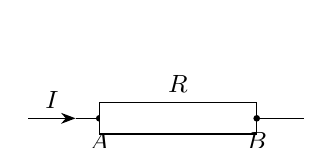
\begin{tikzpicture}[x=1cm,y=1cm,line width=0.5pt,>=Stealth,font=\small]
\draw[->] (-0.9,0)--(-0.3,0) node[midway,above]{$I$}; \draw (-0.3,0)--(0,0); \fill (0,0) circle(1.2pt); \node[below] at (0,-0.05) {$A$};
\draw[fill=white] (0,-0.2) rectangle (2,0.2); \node[above] at (1,0.2) {$R$}; \draw (2,0)--(2.6,0); \fill (2,0) circle(1.2pt); \node[below] at (2,-0.05) {$B$};
\end{tikzpicture}\par\smallskip
\opt{A}{7}
\opt{B}{$-$12}
\opt{C}{$-$7}
\opt{D}{12}
\end{minipage}\vspace{9pt}\par
\noindent\begin{minipage}{\linewidth}
\textbf{22.}\ Taşqi zanjirga ikkita 2 $\Omega$ va 8 $\Omega$ qarşiliklar ulanganda manbaning foydali quvvati har gal 32 W ga teng bölgan. Manba hosil qilişi mumkin bölgan eng katta foydali quvvatni (W) toping.\par\smallskip
\opt{A}{20}
\opt{B}{32}
\opt{C}{16}
\opt{D}{36}
\end{minipage}\vspace{9pt}\par
\noindent\begin{minipage}{\linewidth}
\textbf{23.}\ Elektroliz vaqtida tok kuçi I = 6 + 0,05t qonun böyiça oqmoqda. 80 s vaqt davomida qanday massali (g) nikel ajralib çiqadi? k = 0,35 $\cdot$ 10$^{-6}$ kg/C\par\smallskip
\opt{A}{0,224}
\opt{B}{0,280}
\opt{C}{0,488}
\opt{D}{0,14}
\end{minipage}\vspace{9pt}\par
\noindent\begin{minipage}{\linewidth}
\textbf{24.}\ Zaryadi q ga teng bölgan nuqtaviy zaryad elektr maydonga kiritildi va unga ta’sir etuvçi kuç q $\cdot$ E ga teng bölsa, bu kuçga aks ta’sir etuvçi kuç nimaga ta’sir etadi?\par\smallskip
\opt{A}{maydonni hosil qiluvçi zaryadlar töplamiga}
\opt{B}{aks ta’sir mavjud emas}
\opt{C}{bu kuç nolga teng}
\opt{D}{zaryadni öziga}
\end{minipage}\vspace{9pt}\par
\noindent\begin{minipage}{\linewidth}
\textbf{25.}\ Nuqtaviy zaryad atrofidagi ikki nuqtada elektr maydon kuçlanganliklari 81 marta farq qiladi. Bu nuqtalardan zaryadgaça bölgan masofalar nisbati qanday?\par\smallskip
\opt{A}{2}
\opt{B}{27}
\opt{C}{9}
\opt{D}{3}
\end{minipage}\vspace{9pt}\par
\noindent\begin{minipage}{\linewidth}
\textbf{26.}\ Nuqtaviy yoruğlik manbaidan 2$\pi$ sr fazoviy burçakda yoruğlik tarqalmoqda. Agar yoruğlik oqimi 12,56 lm bölsa, yoruğlik kuçini toping (cd).\par\smallskip
\opt{A}{2}
\opt{B}{3}
\opt{C}{4}
\opt{D}{5}
\end{minipage}\vspace{9pt}\par
\noindent\begin{minipage}{\linewidth}
\textbf{27.}\ Yiğuvçi linza yordamida ekranda buyumning 2 marta kattalaşgan haqiqiy tasviri hosil qilindi. Buyum va tasvir orasidagi masofa 1,5 m bölsa, linzaning optik kuçini (dptr) aniqlang.\par\smallskip
\opt{A}{3}
\opt{B}{1/3}
\opt{C}{1/4}
\opt{D}{4}
\end{minipage}\vspace{9pt}\par
\noindent\begin{minipage}{\linewidth}
\textbf{28.}\ Yassi közgudan buyumgaça masofa 4 m bölsa, közgudan tasvirgaça masofani aniqlang (m).\par\smallskip
\opt{A}{8}
\opt{B}{2}
\opt{C}{16}
\opt{D}{4}
\end{minipage}\vspace{9pt}\par
\noindent\begin{minipage}{\linewidth}
\textbf{29.}\ Tomoni 1 m ga teng bölgan kvadrat şaklidagi juda yupqa plastinka öz tekisligida yotgan va bir tomoniga parallel bölgan yönaliş böyiça $0{,}8c$ tezlik bilan harakatlanmoqda. Tinç turgan kuzatuvçiga nisbatan kvadrat yuzasi qanday böladi (m$^{2}$)?\par\smallskip
\opt{A}{1}
\opt{B}{0,7}
\opt{C}{0,36}
\opt{D}{0,6}
\end{minipage}\vspace{9pt}\par
\noindent\begin{minipage}{\linewidth}
\textbf{30.}\ Natriyning elektrokimyoviy ekvivalentini aniqlang (mg/C). Natriy atom massasi A=0,023 kg/mol, valentligi z=1. F=96500 C/mol.\par\smallskip
\opt{A}{0,329}
\opt{B}{0,125}
\opt{C}{0,568}
\opt{D}{0,238}
\end{minipage}\vspace{9pt}\par
\noindent\begin{minipage}{\linewidth}
\textbf{31.}\ Köp atomli gaz molekulalarining erkinlik darajasi i = 6. Özgarmas hajmda şu gazning molyar issiqlik siğimini aniqlang.\par\smallskip
\opt{A}{4R}
\opt{B}{3R}
\opt{C}{R}
\opt{D}{1,5R}
\end{minipage}\vspace{9pt}\par
\noindent\begin{minipage}{\linewidth}
\textbf{32.}\ Odam 5 m oldinga harakatlanib, söngra 4 m orqaga yuridi. Uning köçişini (m) aniqlang.\par\smallskip
\opt{A}{9}
\opt{B}{5}
\opt{C}{4}
\opt{D}{1}
\end{minipage}\vspace{9pt}\par
\newpage\noindent\textbf{33–35-test topşiriqlariga mos keluvçi javoblarni (A–F) javob variantlaridan tanlang.}\par\smallskip
Nominal kuçlanişi 120 V bölgan ikkita isitgiçning nominal quvvatlari $P_1=360$ W va $P_2=180$ W. Isitgiçlar ketma-ket ulanib, 120 V kuçlanişli tarmoqqa ulandi (rasm). Qarşiliklar özgarmas deb hisoblansin.\par\medskip
\begin{center}\begin{tikzpicture}[x=1cm,y=1cm,line width=0.5pt,>=Stealth,font=\small]
\draw (0,0.3)--(0,0)--(4.6,0)--(4.6,1.6)--(4.0,1.6); \draw (0,0.6)--(0,1.6)--(0.9,1.6);
\draw (-0.3,0.6)--(0.3,0.6); \draw (-0.15,0.3)--(0.15,0.3); \node[left] at (-0.35,0.45) {$U$};
\draw[fill=white] (0.9,1.45) rectangle (1.9,1.75); \node[above] at (1.4,1.75) {$R_1$}; \draw (1.9,1.6)--(3.0,1.6);
\draw[fill=white] (3.0,1.45) rectangle (4.0,1.75); \node[above] at (3.5,1.75) {$R_2$};
\end{tikzpicture}\end{center}
\noindent\fbox{\begin{minipage}{0.64\linewidth}\vspace{4pt}\textbf{33.}\ Zanjirdagi tok kuçini (A) toping.\\[6pt]\textbf{34.}\ Birinçi isitgiçda ajralayotgan quvvatni (W) toping.\\[6pt]\textbf{35.}\ Isitgiçlar şu tarmoqqa parallel ulanganda umumiy quvvatni (W) toping.\vspace{4pt}\end{minipage}\vrule\hspace{6pt}\begin{minipage}{0.28\linewidth}\vspace{4pt}A)\ 1\\B)\ 3\\C)\ 40\\D)\ 120\\E)\ 270\\F)\ 540\vspace{4pt}\end{minipage}}\par\vspace{14pt}
\Needspace{9\baselineskip}
\noindent\textbf{36.}\ Kesim yuzalari bir xil bölgan U simon nayçada suv bor. Nayçaning bir tirsagiga 20 cm balandlikda kerosin quyildi. $\rho_{kerosin}=800$ kg/m$^3$.\par\smallskip
\medskip\noindent\textbf{a)\ Ikkala tirsakdagi suyuqlik sathlarining farqini (cm) toping.}\par
\noindent\textit{Javob}: a)\ \blank\par
\medskip\noindent\textbf{b)\ Ikkinçi tirsakdagi suv sathi dastlabki holatiga nisbatan neça santimetrga kötarildi?}\par
\noindent\textit{Javob}: b)\ \blank\par
\medskip\noindent\textbf{Diqqat!} Javoblaringizni javoblar varaqasiga köçirib yozing.\par\vspace{10pt}
\Needspace{9\baselineskip}
\noindent\textbf{37.}\ Avtomobil tinç holatdan tekis tezlanuvçan harakatlanib, 10 s da 20 m/s tezlikka erişdi, söngra 4 m/s$^2$ tezlaniş bilan tormozlanib töxtadi.\par\smallskip
\medskip\noindent\textbf{a)\ Avtomobilning butun harakat vaqtini (s) toping.}\par
\noindent\textit{Javob}: a)\ \blank\par
\medskip\noindent\textbf{b)\ Avtomobilning butun harakat davomida bosib ötgan yölini (m) toping.}\par
\noindent\textit{Javob}: b)\ \blank\par
\medskip\noindent\textbf{Diqqat!} Javoblaringizni javoblar varaqasiga köçirib yozing.\par\vspace{10pt}
\Needspace{9\baselineskip}
\noindent\textbf{38.}\ Massasi 70 kg bölgan odam liftda turibdi. $g=10$ m/s$^2$.\par\smallskip
\medskip\noindent\textbf{a)\ Lift 2 m/s$^2$ tezlaniş bilan yuqoriga tezlanib kötarilayotganda odamning oğirligini (N) toping.}\par
\noindent\textit{Javob}: a)\ \blank\par
\medskip\noindent\textbf{b)\ Lift 2 m/s$^2$ tezlaniş bilan pastga tezlanib tuşayotganda odamning oğirligini (N) toping.}\par
\noindent\textit{Javob}: b)\ \blank\par
\medskip\noindent\textbf{Diqqat!} Javoblaringizni javoblar varaqasiga köçirib yozing.\par\vspace{10pt}
\Needspace{9\baselineskip}
\noindent\textbf{39.}\ Ideal gaz molekulalarining temperaturasi 300 K. $k=1{,}38\cdot10^{-23}$ J/K.\par\smallskip
\medskip\noindent\textbf{a)\ Molekulalar ilgarilanma harakatining örtaça kinetik energiyasini ($10^{-21}$ J) toping.}\par
\noindent\textit{Javob}: a)\ \blank\par
\medskip\noindent\textbf{b)\ Qanday temperaturada (K) bu energiya 2 marta ortadi?}\par
\noindent\textit{Javob}: b)\ \blank\par
\medskip\noindent\textbf{Diqqat!} Javoblaringizni javoblar varaqasiga köçirib yozing.\par\vspace{10pt}
\Needspace{9\baselineskip}
\noindent\textbf{40.}\ 0 $^\circ$C temperaturali muz bölagi 55 $^\circ$C temperaturali 2 kg suvga solindi va muz töliq erib, aralaşma temperaturasi 0 $^\circ$C böldi. $c_{suv}=4200$ J/(kg$\cdot$K), $\lambda_{muz}=330$ kJ/kg.\par\smallskip
\medskip\noindent\textbf{a)\ Suv bergan issiqlik miqdorini (kJ) toping.}\par
\noindent\textit{Javob}: a)\ \blank\par
\medskip\noindent\textbf{b)\ Muzning massasini (kg) toping.}\par
\noindent\textit{Javob}: b)\ \blank\par
\medskip\noindent\textbf{Diqqat!} Javoblaringizni javoblar varaqasiga köçirib yozing.\par\vspace{10pt}
\Needspace{9\baselineskip}
\noindent\textbf{41.}\ EYuK 12 V, içki qarşiligi 0,5 $\Omega$ bölgan tok manbaiga 5,5 $\Omega$ li taşqi qarşilik ulangan.\par\smallskip
\medskip\noindent\textbf{a)\ Zanjirdagi tok kuçini (A) toping.}\par
\noindent\textit{Javob}: a)\ \blank\par
\medskip\noindent\textbf{b)\ Qisqa tutaşuv tokini (A) toping.}\par
\noindent\textit{Javob}: b)\ \blank\par
\medskip\noindent\textbf{Diqqat!} Javoblaringizni javoblar varaqasiga köçirib yozing.\par\vspace{10pt}
\Needspace{9\baselineskip}
\noindent\textbf{42.}\ Yassi havo kondensatori qoplamalarining yuzasi 200 cm$^2$, ular orasidagi masofa 1 mm. Kondensator 100 V kuçlanişli manbaga ulangan. $\varepsilon_0=8{,}85\cdot10^{-12}$ F/m.\par\smallskip
\medskip\noindent\textbf{a)\ Kondensator siğimini (pF) toping.}\par
\noindent\textit{Javob}: a)\ \blank\par
\medskip\noindent\textbf{b)\ Kondensator qoplamalaridagi zaryadni (nC) toping.}\par
\noindent\textit{Javob}: b)\ \blank\par
\medskip\noindent\textbf{Diqqat!} Javoblaringizni javoblar varaqasiga köçirib yozing.\par\vspace{10pt}
\Needspace{9\baselineskip}
\noindent\textbf{43.}\ Böyi 1,8 m bölgan odamning közlari poldan 1,7 m balandlikda. Odam vertikal yassi közguga qarab turibdi.\par\smallskip
\medskip\noindent\textbf{a)\ Odam özini töliq körişi uçun közguning eng kiçik balandligini (m) toping.}\par
\noindent\textit{Javob}: a)\ \blank\par
\medskip\noindent\textbf{b)\ Bunda közguning pastki qirrasi poldan qanday balandlikda (m) bölişi kerak?}\par
\noindent\textit{Javob}: b)\ \blank\par
\medskip\noindent\textbf{Diqqat!} Javoblaringizni javoblar varaqasiga köçirib yozing.\par\vspace{10pt}
\Needspace{9\baselineskip}
\noindent\textbf{44.}\ Optik kuçlari $+5$ dptr va $-1$ dptr bölgan ikkita yupqa linza bir-biriga ziç tegib turibdi.\par\smallskip
\medskip\noindent\textbf{a)\ Linzalar sistemasining optik kuçini (dptr) toping.}\par
\noindent\textit{Javob}: a)\ \blank\par
\medskip\noindent\textbf{b)\ Sistemaning fokus masofasini (cm) toping.}\par
\noindent\textit{Javob}: b)\ \blank\par
\medskip\noindent\textbf{Diqqat!} Javoblaringizni javoblar varaqasiga köçirib yozing.\par\vspace{10pt}
\Needspace{9\baselineskip}
\noindent\textbf{45.}\ $^{238}_{92}$U yadrosi bir qator radioaktiv yemirilişlardan söng $^{206}_{82}$Pb yadrosiga aylandi.\par\smallskip
\medskip\noindent\textbf{a)\ Neça marta $\alpha$-yemiriliş sodir bölgan?}\par
\noindent\textit{Javob}: a)\ \blank\par
\medskip\noindent\textbf{b)\ Neça marta $\beta$-yemiriliş sodir bölgan?}\par
\noindent\textit{Javob}: b)\ \blank\par
\medskip\noindent\textbf{Diqqat!} Javoblaringizni javoblar varaqasiga köçirib yozing.\par\vspace{10pt}
\end{document}